\documentclass[10pt]{beamer}

\usetheme{metropolis}
\usepackage{appendixnumberbeamer}

\usepackage{booktabs}
\usepackage[scale=2]{ccicons}
\usepackage{graphicx}
\usepackage{hyperref}
\usepackage{circuitikz}
\usepackage{pdflscape}
\usepackage{smartdiagram}

\usepackage{color}
\usepackage{listings}

\lstset{
	basicstyle=\footnotesize\ttfamily,
    keepspaces=true,
    showstringspaces=false,
    language=PHP,
    commentstyle=\ttfamily,
}

\usepackage[OT4]{polski}
\usepackage[utf8]{inputenc}

\usepackage{pgfplots}
\usepgfplotslibrary{dateplot}

\usepackage{xspace}
\newcommand{\themename}{\textbf{\textsc{metropolis}}\xspace}

\setbeamertemplate{frame footer}{}
\setbeamertemplate{frame numbering}{}

\usetikzlibrary{shapes,arrows}

\tikzstyle{decision} = [diamond, draw, fill=blue!20, 
    text width=4.5em, text badly centered, node distance=3cm, inner sep=0pt]
\tikzstyle{block} = [rectangle, draw, fill=blue!20, 
    text width=5em, text centered, rounded corners, minimum height=4em]
\tikzstyle{line} = [draw, -latex']
\tikzstyle{cloud} = [draw, ellipse,fill=red!20, node distance=3cm,
    minimum height=2em]


\title{Praktyczny polimorfizm}

\subtitle{Projektowanie i programowanie systemów internetowych I}
\author{mgr inż. Krzysztof Rewak}
\date{\today}
\institute{Wydział Nauk Technicznych i Ekonomicznych \\ Państwowa Wyższa Szkoła Zawodowa im. Witelona w Legnicy}

\begin{document}

\maketitle

\begin{frame}{Plan prezentacji}
  \setbeamertemplate{section in toc}[sections numbered]
  \tableofcontents[hideallsubsections]
\end{frame}


\section{Polimorfizm}

\begin{frame}{Definicja}
	Czym jest polimorfizm?
\end{frame}

\begin{frame}{Definicja}
	Z greki \emph{wielopostaciowość}, polimorfizm to umożliwienie jednym sposobem dostępu do wielu różnych \emph{wartości}.
\end{frame}

\begin{frame}{Definicja}
	Wykorzystanie polimorfizmu może być jednym z podstawowych narzędzi refaktoryzacji kodu w celu uzyskania tzw. czystego kodu.
\end{frame}

\begin{frame}{Definicja}
	Wykorzystanie polimorfizmu powinno natomiast być podstawowym narzędziem przy planowaniu architektury aplikacji, zarówno na poziomie całego projektu, jak i jego części.
\end{frame}

\section{Polimorfizm \emph{ad hoc}}

\begin{frame}{Definicja}
	Tzw. polimorfizm \emph{ad hoc} to sposób na wywoływanie określonych funkcji na argumentach wybranego typu.
\end{frame}

\begin{frame}{Przeciążanie operatorów}
	Jednym z narzędzi polimorfizmu \emph{ad hoc} jest przeciążanie operatorów, o którym była już mowa na zajęciach z Projektowania i programowania obiektowego I.
\end{frame}

\begin{frame}
	\begin{figure} \centering
		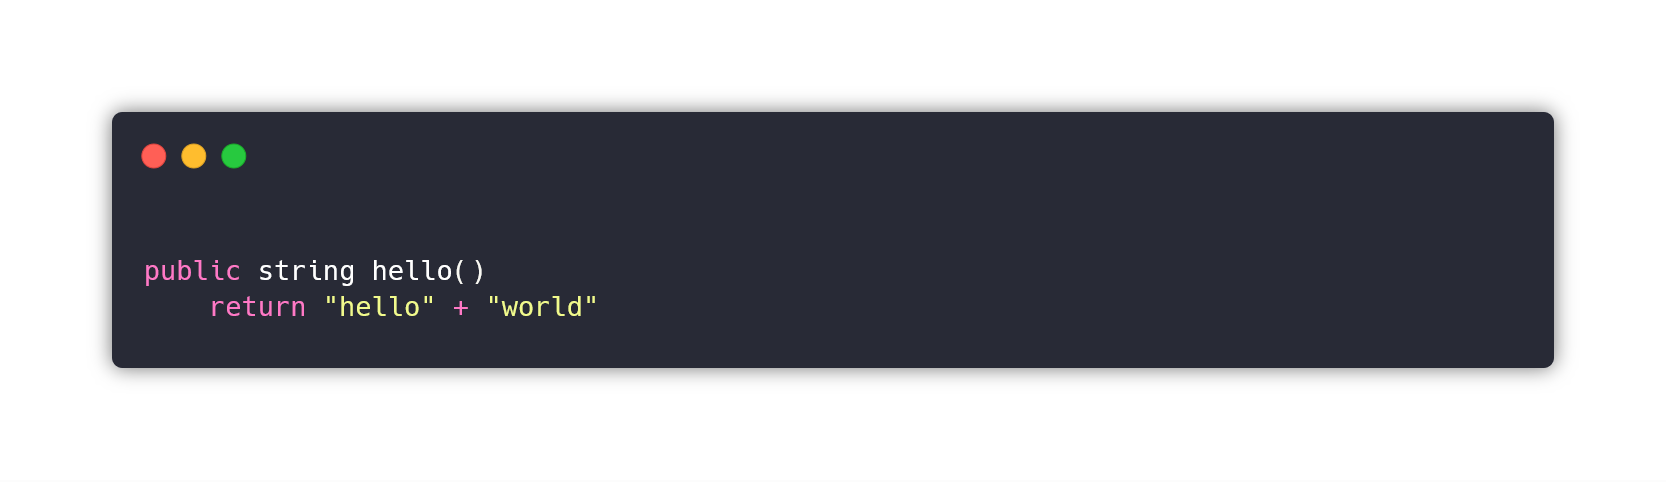
\includegraphics[width=\textwidth]{hello.png}
	\end{figure}
\end{frame}

\begin{frame}
	\begin{figure} \centering
		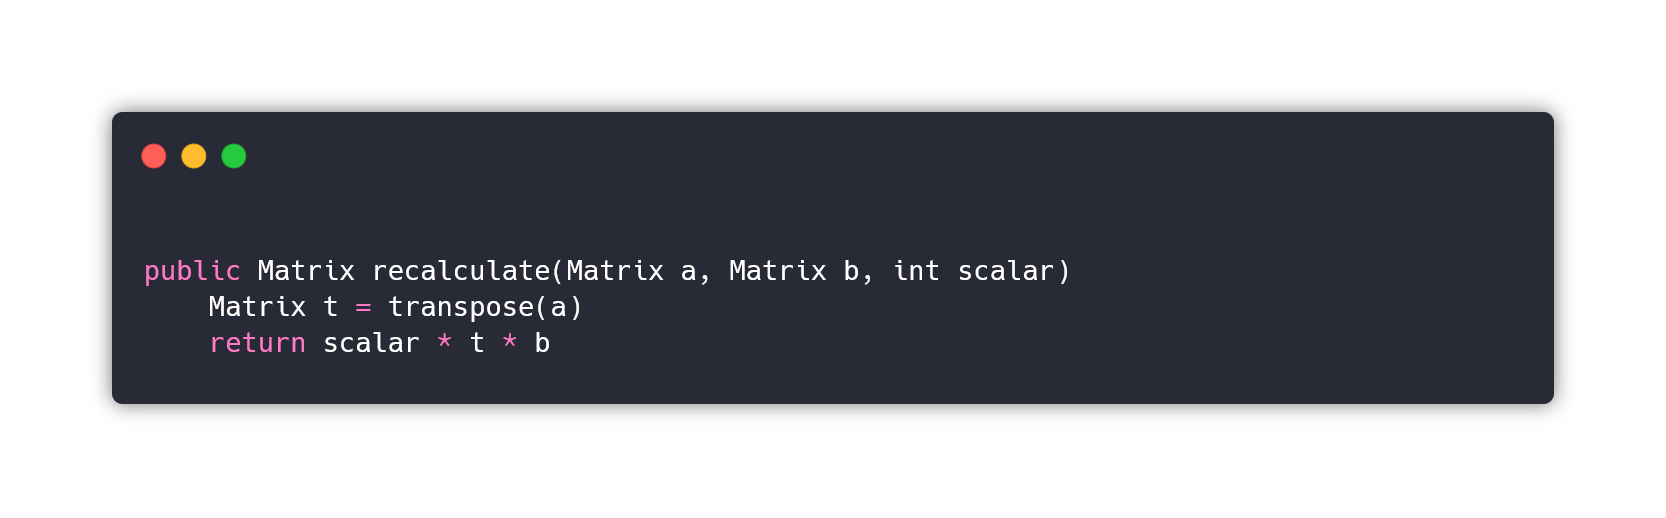
\includegraphics[width=\textwidth]{matrix.png}
	\end{figure}
\end{frame}

\begin{frame}
	\begin{figure} \centering
		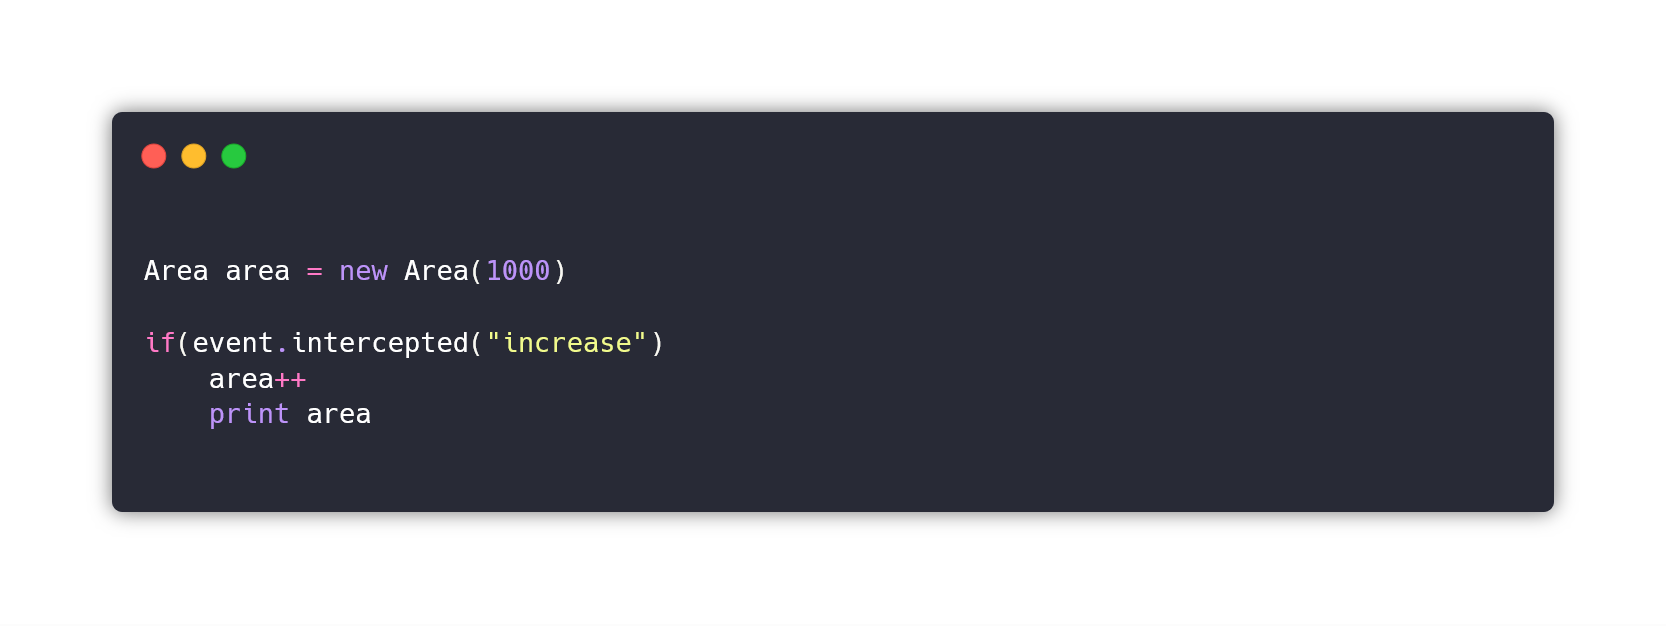
\includegraphics[width=\textwidth]{oo.png}
	\end{figure}
\end{frame}

\begin{frame}
	\begin{figure} \centering
		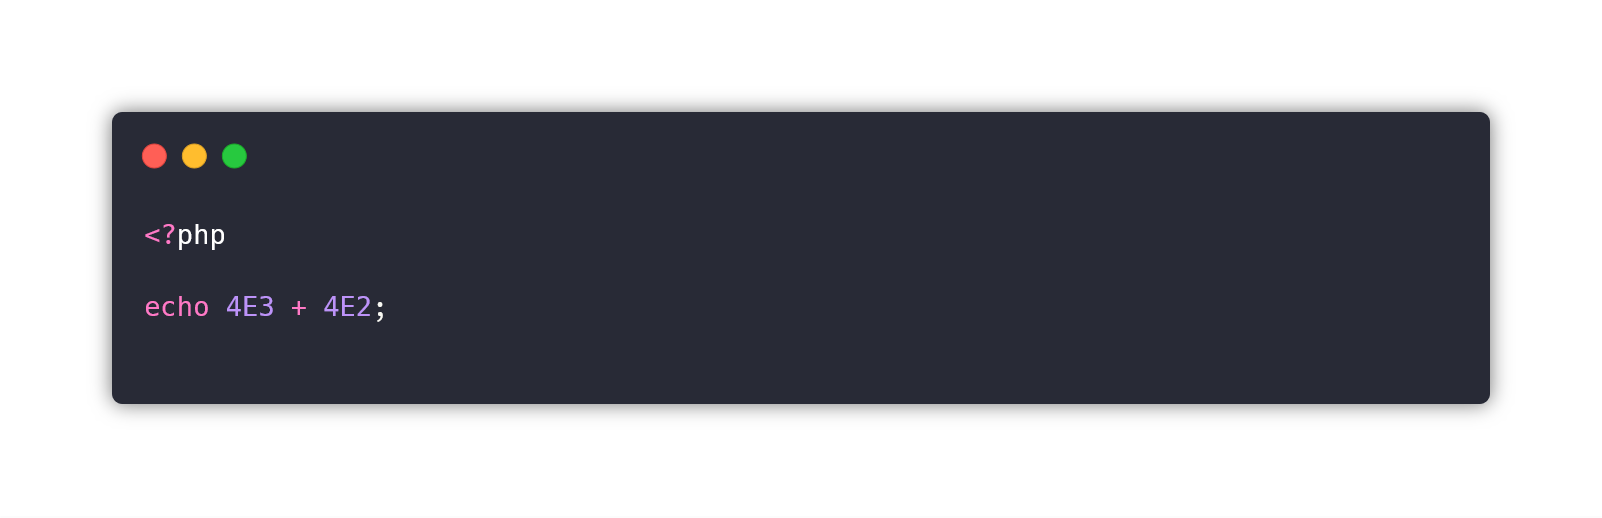
\includegraphics[width=\textwidth]{4400.png}
	\end{figure}
\end{frame}

\begin{frame}{Przeciążanie operatorów}
	Przeciążanie operatorów jest często nazywane \emph{składniowym lukrem}. Oznacza to, że taka konstrukcja istnieje tylko i wyłącznie dla wygody programisty.
	
	Ale czy lukier jest zdrowy?
\end{frame}

\begin{frame}{Przeciążanie funkcji}
	Niektóre języki programowania pozwalają na tworzenie wielu różnie zaimplementowanych funkcji o tej samej nazwie. Na podstawie typów przekazanych parametrów wybierana jest konkretna implementacja do wywołania.
\end{frame}

\begin{frame}
	\begin{figure} \centering
		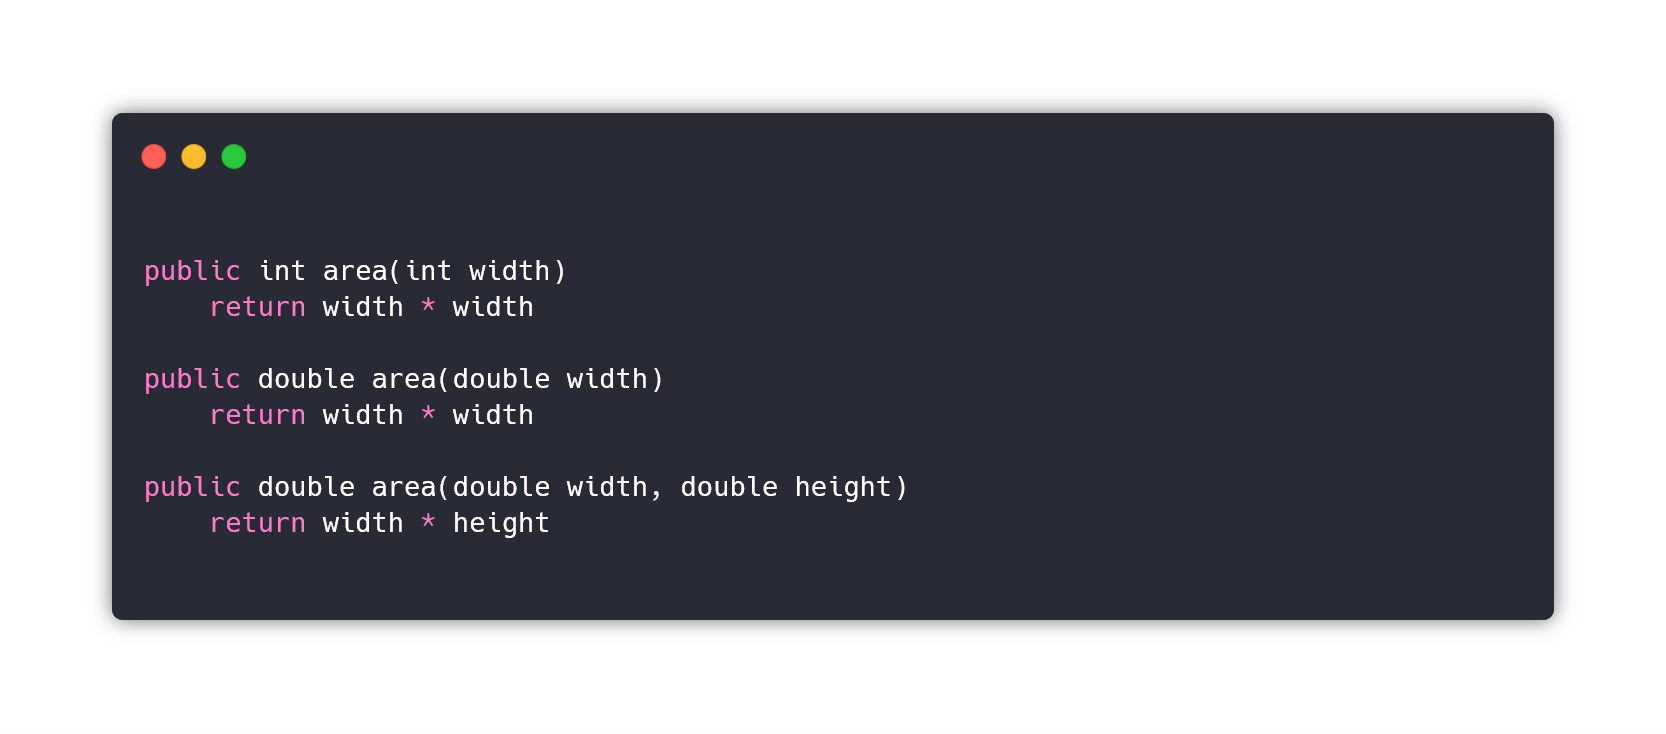
\includegraphics[width=\textwidth]{fo.png}
	\end{figure}
\end{frame}

\begin{frame}{Koercja}
	Większość języków programowania dopuszcza tzw. rzutowanie typów. Czy wymuszoną konwersję jednego typu na drugi można nazwać implementacją polimorfizmu?
\end{frame}

\begin{frame}
	\begin{figure} \centering
		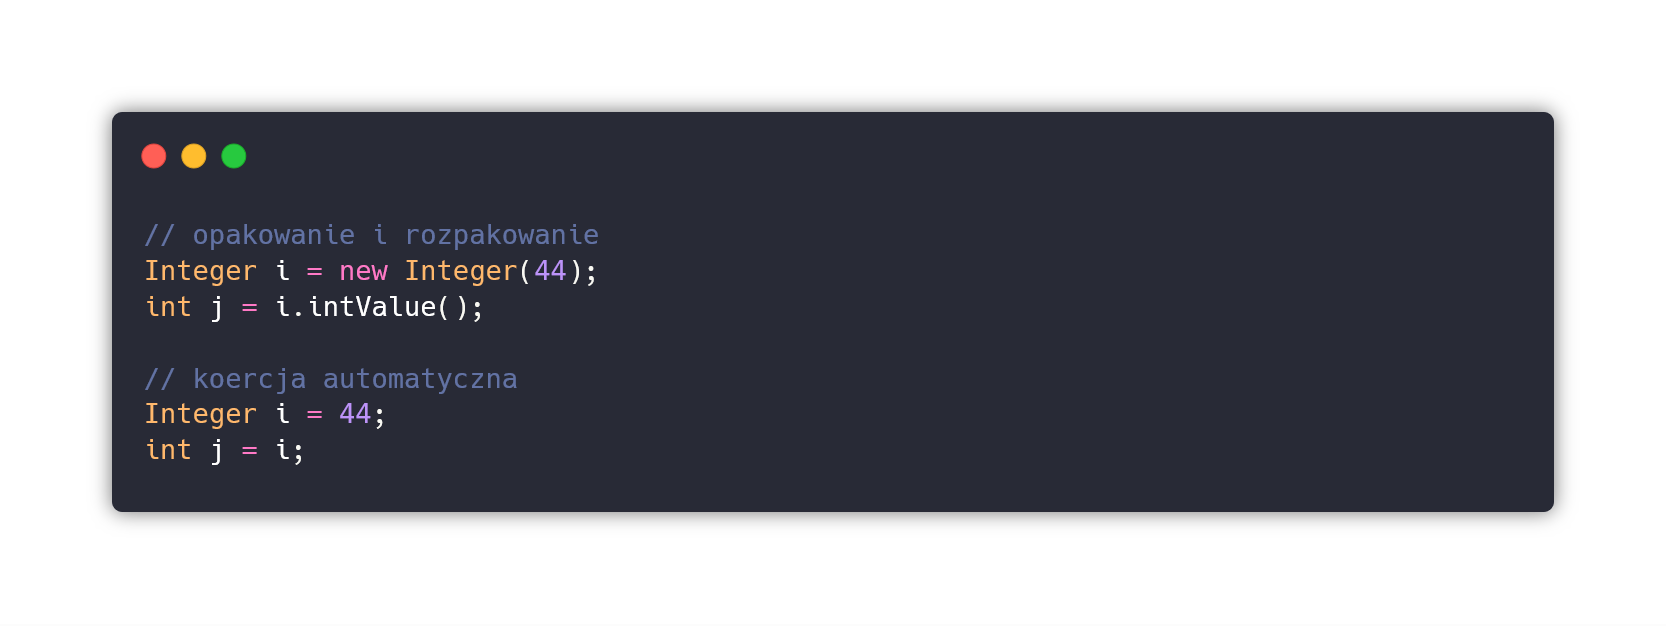
\includegraphics[width=\textwidth]{koercja.png}
	\end{figure}
\end{frame}

\begin{frame}{Definicja}
	Czym zatem jest polimorfizm \emph{ad hoc}? I dlaczego jest \emph{ad hoc}?
\end{frame}

\section{Polimorfizm uniwersalny}

\begin{frame}{Definicja}
	Polimorfizm uniwersalny, za Wikipedią, pozwala pisać ogólne struktury danych i algorytmy, bez precyzowania na jakich dokładnie typach one operują i bez konieczności dostarczania implementacji odpowiednich dla każdego przypadku. 
	
	\footnotesize{\url{https://pl.wikipedia.org/wiki/Polimorfizm_(informatyka)}}
\end{frame}

\begin{frame}{Polimorfizm parametryczny}
	Niektóre języki programowania pozwalają na tworzenie tzw. typów generycznych, które pozwalają na wykorzystywanie danych bez względu na ich typ, a zależnie od zaimplementowanego interfejsu.
\end{frame}

\begin{frame}
	\begin{figure} \centering
		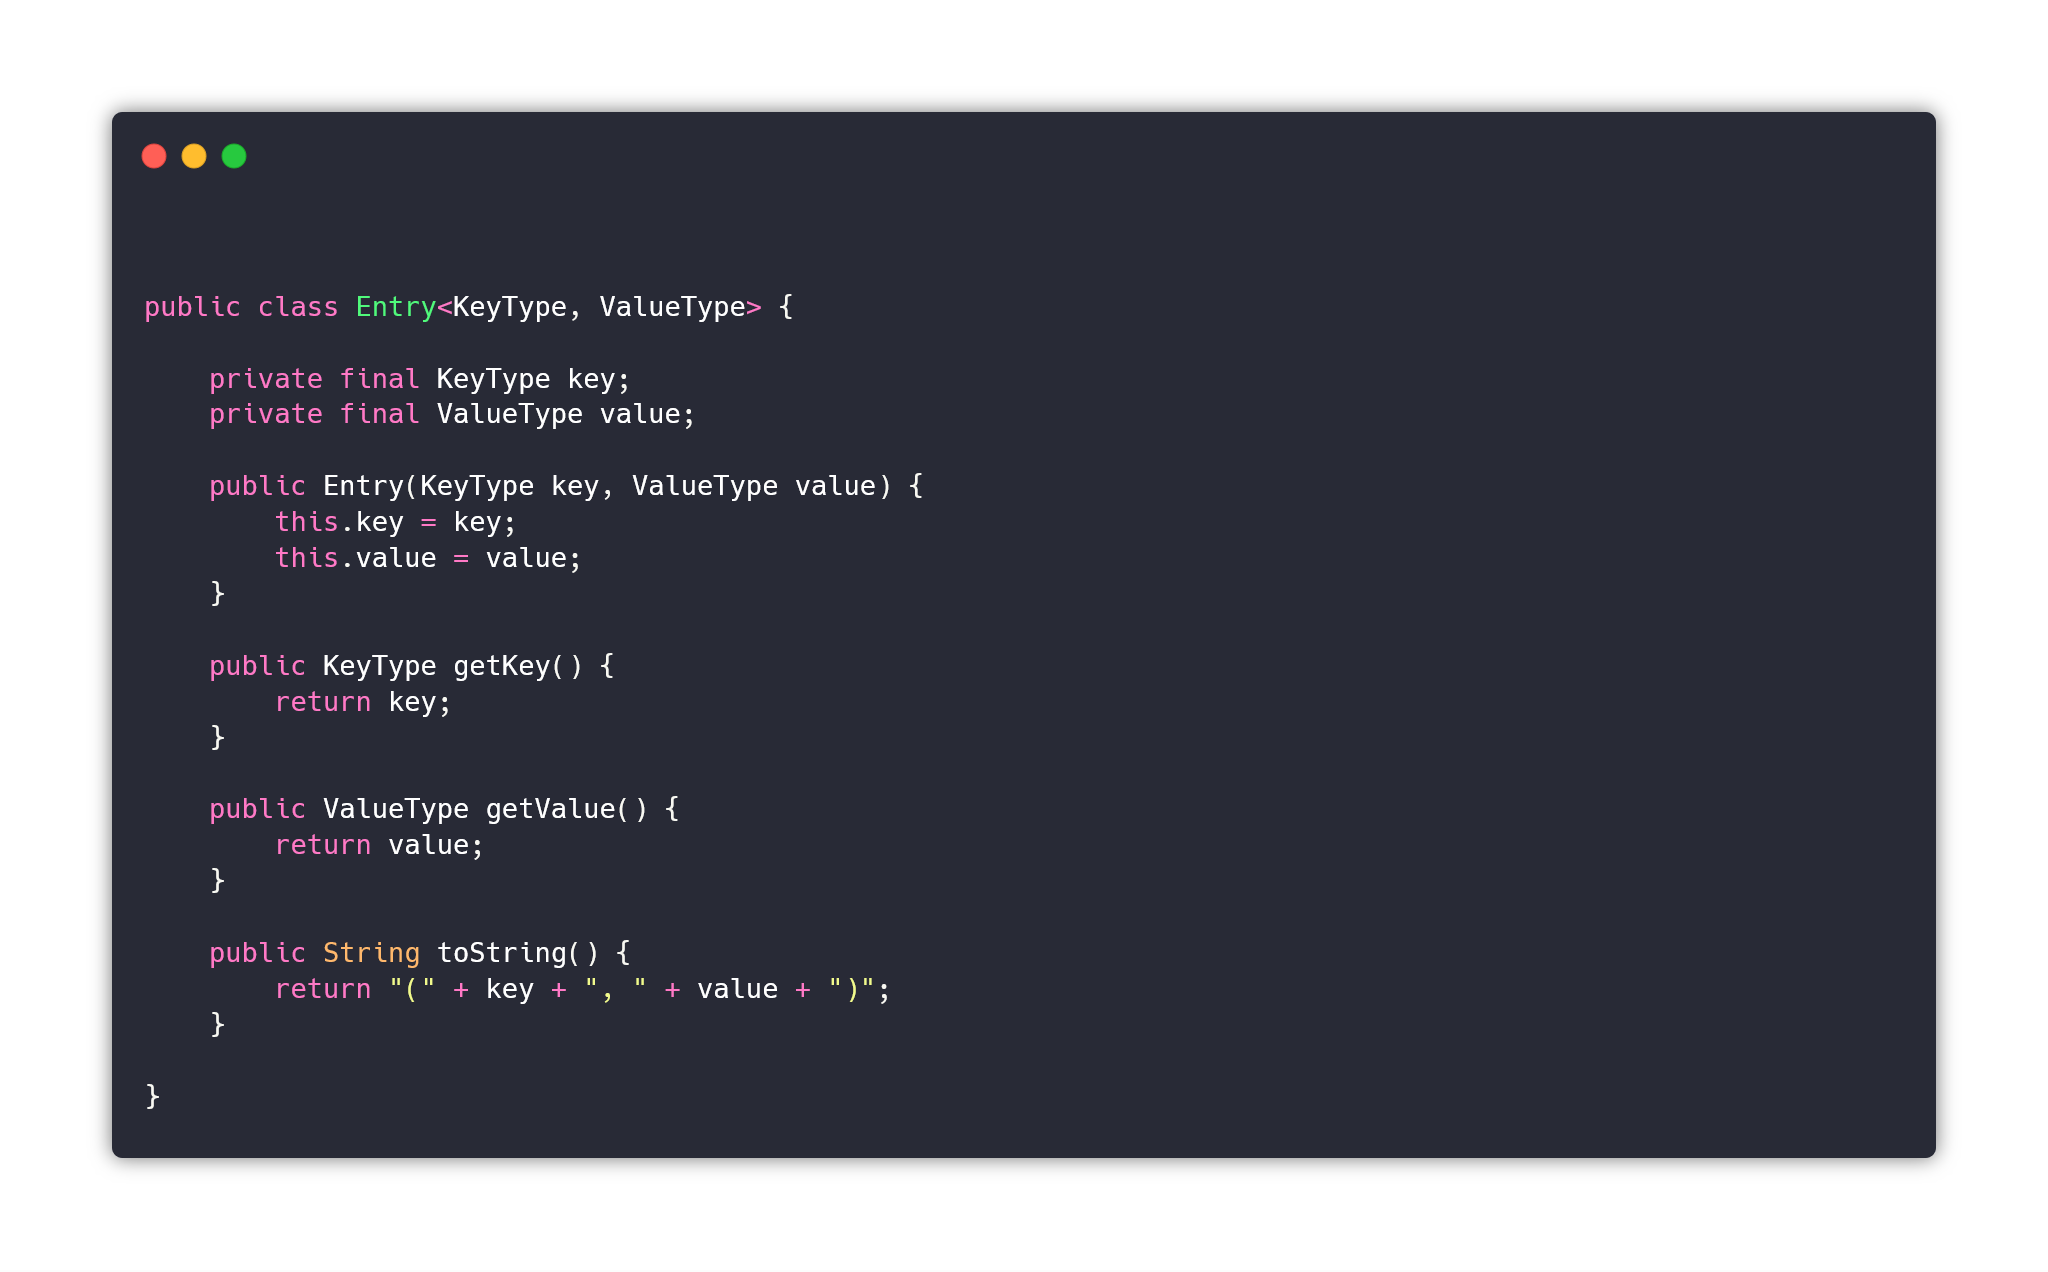
\includegraphics[width=\textwidth]{java.png}
	\end{figure}
\end{frame}

\begin{frame}{Polimorfizm parametryczny}
	Czy takie rozwiązanie różni się od wcześniej przedstawionych przykładów?
\end{frame}

\begin{frame}{Polimorfizm parametryczny}
	Jak można wykorzystać polimorfizm do refaktoryzacji kodu?
\end{frame}

\begin{frame}
	\begin{figure} \centering
		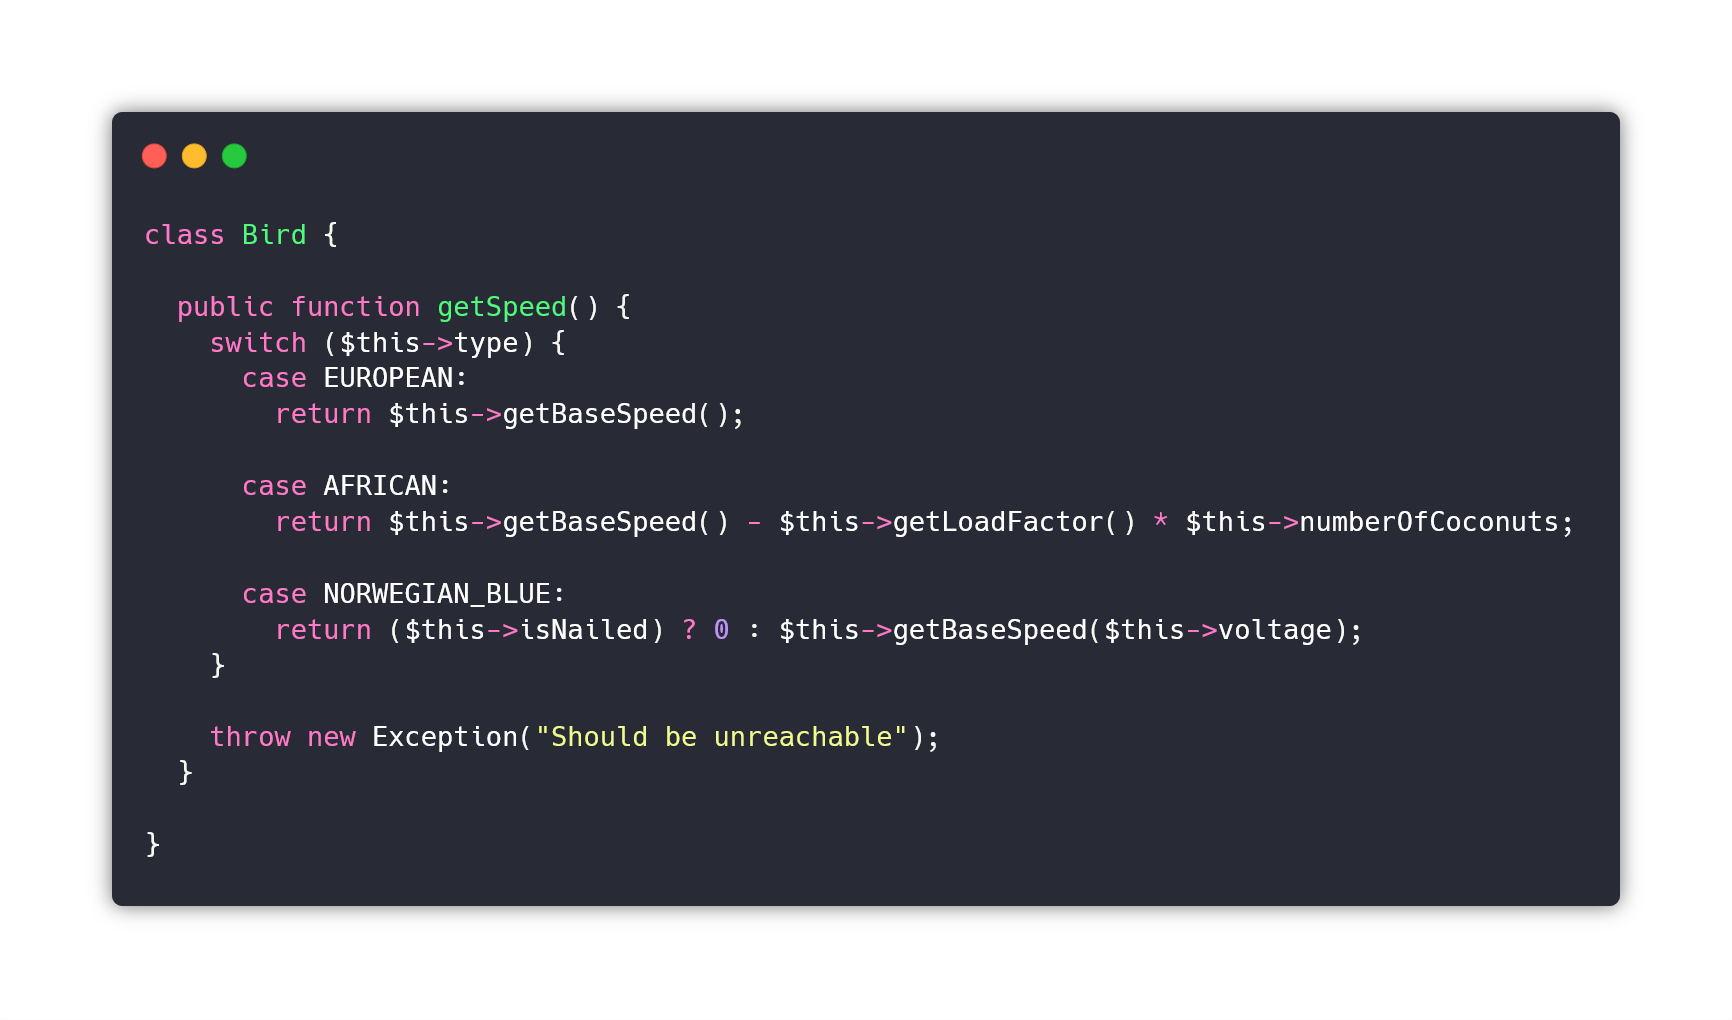
\includegraphics[width=\textwidth]{birds.png}
		\footnotesize{przykład za \url{https://refactoring.guru/replace-conditional-with-polymorphism}}
	\end{figure}
\end{frame}

\begin{frame}
	\begin{figure} \centering
		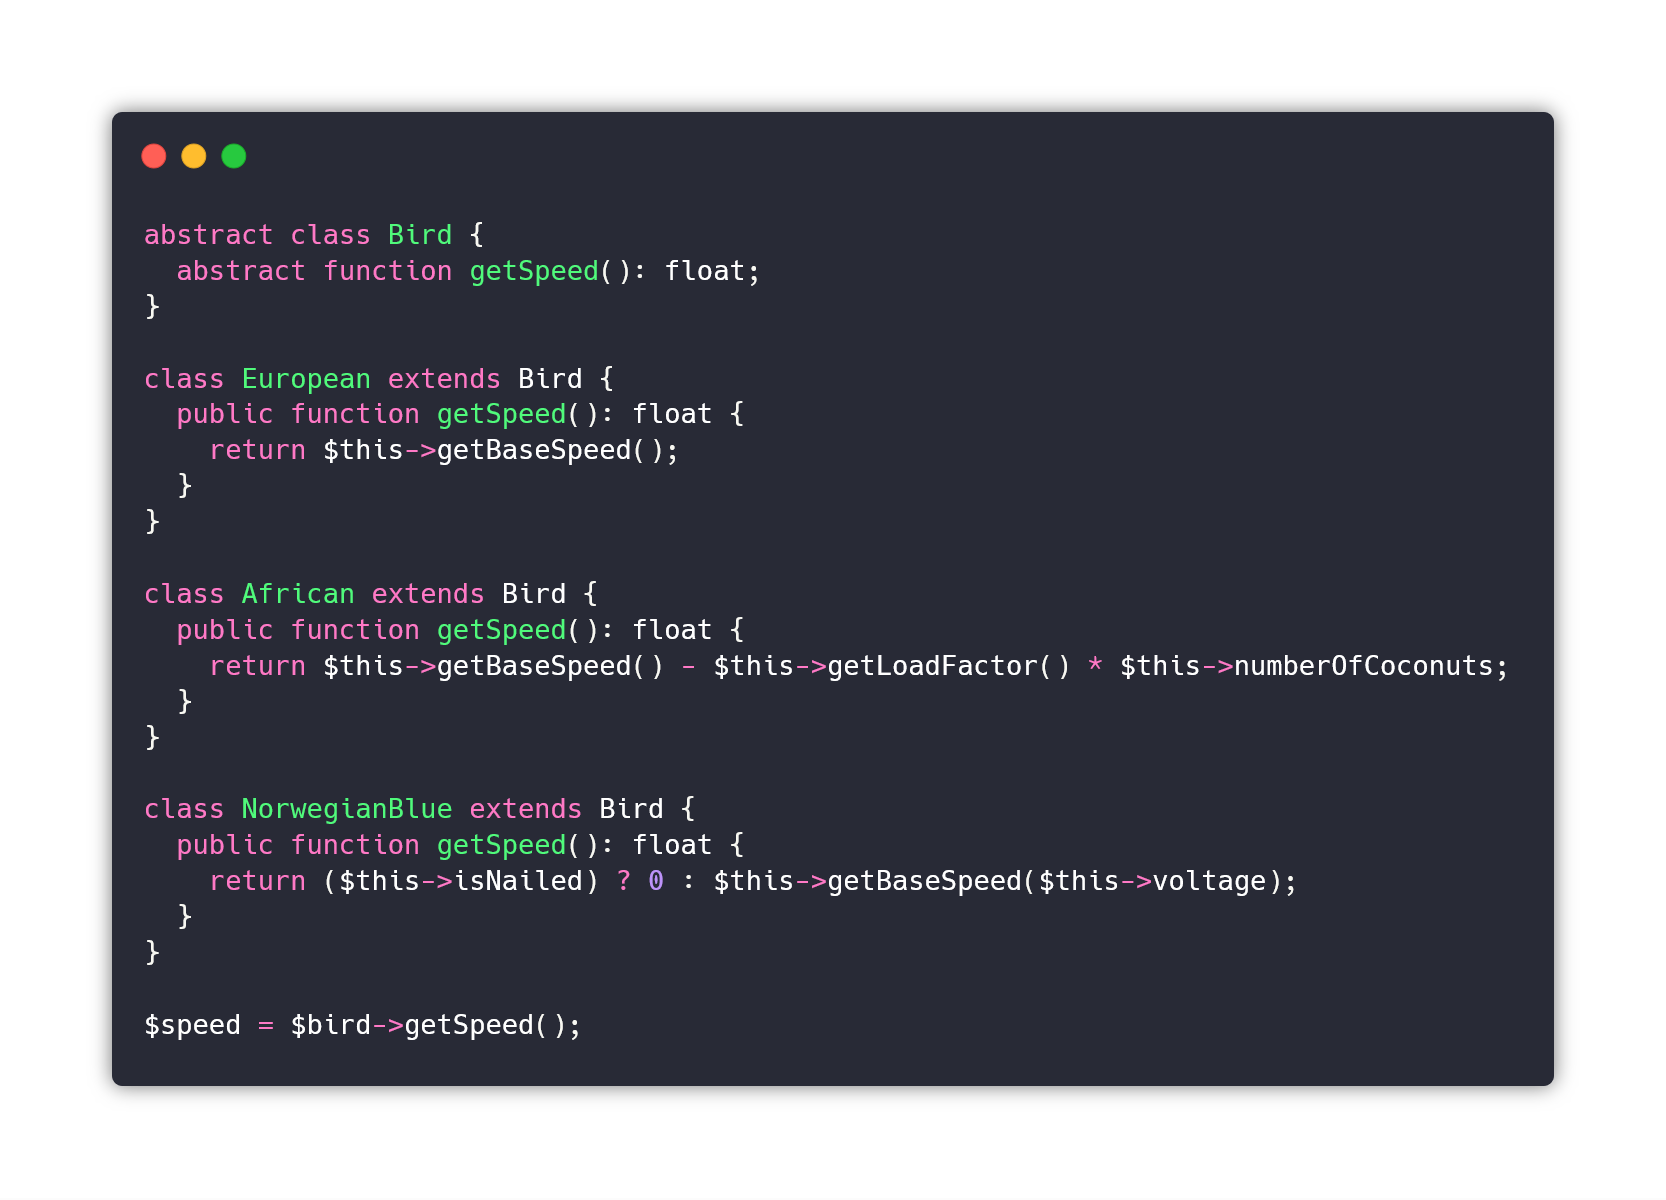
\includegraphics[width=\textwidth]{birds2.png}
		\footnotesize{przykład za \url{https://refactoring.guru/replace-conditional-with-polymorphism}}
	\end{figure}
\end{frame}

\begin{frame}{Polimorfizm parametryczny}
	Powinniśmy stwierdzić, że drugie rozwiązanie nie tylko ładnie obrazuje metodę \emph{Tell, Don't Ask}, ale także spełnia warunek \emph{Open/Closed Principle}. 
\end{frame}

\section{Podsumowanie}

\begin{frame}{Bibliografia i ciekawe źródła}
  
	\begin{thebibliography}{9}
		
		\bibitem{ii}
		\url{www.ii.uni.wroc.pl/~zs/Dydaktyka/TPJP/JavaPolimorfizm.pdf}
		
		\bibitem{wiki}
		\url{https://en.wikipedia.org/wiki/Parametric_polymorphism}
		
		\bibitem{refactoring}
		\url{https://refactoring.guru/replace-conditional-with-polymorphism}
		
	\end{thebibliography}

\end{frame}

\appendix

\begin{frame}[standout]
	Pytania?
\end{frame}

\begin{frame}{}

	Kod prezentacji dostępny jest w repozytorium git pod adresem \texttt{https://bitbucket.org/krewak/pwsz-ppsi} \\ \ \\

	\begin{figure}
		\centering
		\href{https://bitbucket.org/krewak/pwsz-ppsi}{
			
\includegraphics[width=.15\textwidth]{../_template/bitbucket.png}
		}
	\end{figure}
	
	Wszystkie informacje dot. kursu dostępne są pod adresem \texttt{http://pwsz.rewak.pl/kursy/4} \\ \ \\

	\begin{figure}
		\centering
		\href{http://pwsz.rewak.pl/kursy/3}{
			
\includegraphics[width=.15\textwidth]{../_template/rewak.png}
		}
	\end{figure}

\end{frame}

\end{document}
